\section{Web3} 
web3.js is a collection of libraries that allow you to interact with a local or remote Ethereum node. Moreover, it is able to communicate with MetaMask, which is the add-on for Chrome and Mozilla Firefox that lets the user manage his Ethereum wallet and confirm transactions in an intuitive and secure way. Using MetaMask we offer secure payments and automatic login.
\subsection{Architecture overview}
To interact with web3 library calls we organized the \texttt{web3functions} package into five different modules:
\begin{figure}[h]
	\centering
	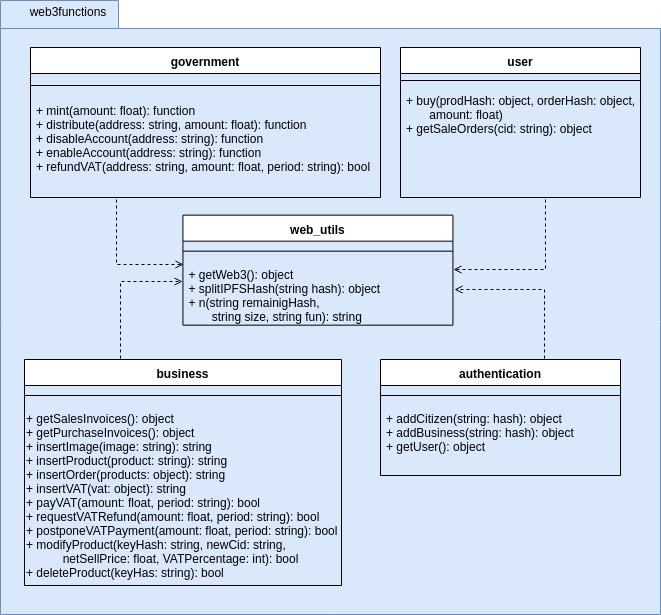
\includegraphics[scale=0.65]{res/images/web3.png}
	\caption{Class diagram of the \texttt{web3functions} package}
\end{figure}
\subsection{Methods}

The 5 modules groups some methods that are responsible for setting data to Ethereum or retrieving them from the blockchain.

\subsubsection{web\_utils}
This module group some utility functions that are used by the other modules to make the web3 call easier:
\begin{itemize}
	\item \textbf{getWeb3}: tries to get an instance of a web3 object, which will be used to make all the web3 calls. Specifically, it tries to get the web3 object instance injected by MetaMask, if this is possible, otherwise it returns an error;
	\item \textbf{splitIPFSHash}: a function that converts the base58 string representing the IPFS CID into three variables, since this information is saved in this way in the blockchain for cost and scalability reasons;
	\item \textbf{recomposeIPFSHash}: a function that does the inverse of the above-descripted function, to recompose the IPFS CID.
\end{itemize} 

\subsubsection{authentication}
Module to manage the registration and login of all the types of users:
\begin{itemize}
	\item \textbf{addCitizen}: registers a new citizen using the Ethereum address provided by MetaMask, and saves the IPFS CID, that represents the related information saved in the peer-to-peer network;
	\item \textbf{addBusiness}: registers a new business using the Ethereum address provided by MetaMask, and saves the IPFS CID, that represents the related information saved in the peer-to-peer network;
	\item \textbf{getUser}: returns the IPFS CID corresponding to the current Ethereum address of the user provided by MetaMask.
\end{itemize}
\subsubsection{user}
Module to manage the common functionality offered to citizen and business:
\begin{itemize}
	\item \textbf{buy}: manage a new order making the user transfer the due amount of \textit{Cubit} to the target companies;
	\item \textbf{getSalesOrders}: gets the IPFS CID related to an order. With the IPFS CID all the order's information can be retreived.
\end{itemize}
\subsubsection{business}
Module to manage the functionality offered to business:
\begin{itemize}
	\item \textbf{getSalesInvoices}: returns an array containing all the IPFS CID related to the sales invoices;
	\item \textbf{getPurchaseInvoices}: returns an array containing all the IPFS CID related to the purchases invoices;
	
	\item \textbf{insertProduct}: inserts the product passed as JSON in the Ethereum blockchain; 
	\item \textbf{insertOrder}: creates a new order made of the product passed to the function;
	\item \textbf{insertVAT}: inserts the VAT information related to the order passed to the function;
	\item \textbf{payVAT}: allows a business to pay the VAT owed by the government related to a particular VAT quarter;
	\item \textbf{postponeVATPayment}: allows a business to postpone the VAT payment to the government related to a particular VAT quarter;
	\item \textbf{modifyProduct}: allows a business to modify one of its product that was previously been added;
	\item \textbf{deleteProduct}: allows a business to delete one of its products that were previously been added. The product will not be shown in the store anymore.
\end{itemize}
\subsubsection{government}
Module to manage the common functionality offered to the government:
\begin{itemize}
	\item \textbf{mint}: let the government mint a specific amount of \textit{Cubit}. This amount is deposited in the government account;
	\item \textbf{distribute}: let the government transfer a specific amount of \textit{Cubit} from its account to a target account;
	\item \textbf{disableAccount}: let the government set the state of the target account to "disabled". The target account will not be able to use the platform until it has been restored;
	\item \textbf{modifyProduct}: let the government set the state of the target account to "enabled". The target account will be able to use the platform;
	\item \textbf{refundVAT}: let the government refund a business. The owed amount of \textit{Cubit}, related to a specific VAT quarter, will be transferred to the target business.
\end{itemize}
